\documentclass{article}
\usepackage[utf8]{inputenc}
\usepackage[spanish]{babel}
\usepackage{graphicx}
\usepackage{listings}
\usepackage{color}

\definecolor{codegreen}{rgb}{0,0.6,0}
\definecolor{codegray}{rgb}{0.5,0.5,0.5}
\definecolor{codepurple}{rgb}{0.58,0,0.82}
\definecolor{backcolour}{rgb}{0.95,0.95,0.92}

\lstdefinestyle{mystyle}{
    backgroundcolor=\color{backcolour},   
    commentstyle=\color{codegreen},
    keywordstyle=\color{magenta},
    numberstyle=\tiny\color{codegray},
    stringstyle=\color{codepurple},
    basicstyle=\ttfamily\footnotesize,
    breakatwhitespace=false,         
    breaklines=true,                 
    captionpos=b,                    
    keepspaces=true,                 
    numbers=left,                    
    numbersep=5pt,                  
    showspaces=false,                
    showstringspaces=false,
    showtabs=false,                  
    tabsize=2
}

\lstset{style=mystyle}

\title{Proyecto: Calculadora Aritmética Modular}
\author{José Pablo Donado López}
\date{}

\begin{document}

\maketitle

\section{Descripción general del proyecto}

Este proyecto implementa una Calculadora Aritmética Modular en Python. La calculadora realiza operaciones aritméticas básicas (suma, resta, multiplicación, división y potencia) en el contexto de la aritmética modular, donde todas las operaciones se realizan módulo un número primo p. Además, se han implementado operaciones avanzadas como el cálculo del inverso modular, raíces cuadradas modulares y la resolución de sistemas de congruencias lineales utilizando el Teorema del Resto Chino.

El proyecto consta de tres componentes principales:
\begin{itemize}
    \item Una biblioteca de operaciones modulares básicas
    \item Un módulo de operaciones avanzadas
    \item Una interfaz gráfica de usuario (GUI) para facilitar su uso
\end{itemize}

\section{Explicación de la implementación}

\subsection{Operaciones básicas (operaciones.py)}

Este módulo contiene las funciones para realizar operaciones aritméticas modulares básicas.

\begin{lstlisting}[language=Python]
def mod_add(a: int, b: int, p: int) -> int:
    try:
        validate_inputs(a, b, p)
        result = (a + b) % p
        logging.info(f"Suma modular: {a} + {b} ≡ {result} (mod {p})")
        return result
    except ValueError as e:
        logging.error(f"Error en suma modular: {str(e)}")
        raise
\end{lstlisting}

Cada función valida las entradas, realiza la operación correspondiente y registra el resultado utilizando logging.

\subsection{Operaciones avanzadas (operaciones\_avanzadas.py)}

Este módulo implementa operaciones más complejas como el cálculo del inverso modular y la raíz cuadrada modular.

\begin{lstlisting}[language=Python]
def mod_inverse(a: int, m: int) -> int:
    validate_inputs(a, m, m)
    
    def extended_euclidean(a: int, b: int) -> tuple:
        if a == 0:
            return b, 0, 1
        else:
            gcd, x, y = extended_euclidean(b % a, a)
            return gcd, y - (b // a) * x, x

    gcd, x, _ = extended_euclidean(a, m)
    if gcd != 1:
        raise ValueError(f"El inverso multiplicativo de {a} módulo {m} no existe.")
    else:
        return x % m
\end{lstlisting}

La función \texttt{mod\_inverse} utiliza el algoritmo de Euclides extendido para calcular el inverso multiplicativo modular.

\subsection{Interfaz gráfica (gui.py)}

La interfaz gráfica se implementó utilizando Tkinter, proporcionando una forma fácil de interactuar con la calculadora.

\begin{lstlisting}[language=Python]
class CalculadoraModular:
    def __init__(self, master):
        self.master = master
        master.title("Calculadora Aritmética Modular")

        self.label = tk.Label(master, text="Ingrese la expresión:")
        self.label.pack()

        self.entry = tk.Entry(master)
        self.entry.pack()

        # ... (más código de la interfaz) ...

    def calculate(self):
        try:
            expression = self.entry.get()
            p = int(self.p_entry.get())
            
            if not is_prime(p):
                raise ValueError(f"{p} no es un número primo.")
            
            result = evaluate_expression(expression, p)
            self.result_label.config(text=f"Resultado: {result}")
            logging.info(f"Cálculo exitoso: {expression} ≡ {result} (mod {p})")
        except ValueError as e:
            messagebox.showerror("Error", str(e))
            logging.error(f"Error en la GUI: {str(e)}")
\end{lstlisting}

La clase \texttt{CalculadoraModular} maneja la creación de la interfaz y la lógica para realizar los cálculos.

\section{Capturas de pantalla de la ejecución del programa}
Estructura Inicial del Programa

% Capturas de pantalla de tu programa en ejecución
% \includegraphics[width=0.8\textwidth]{captura2.png}
% 1
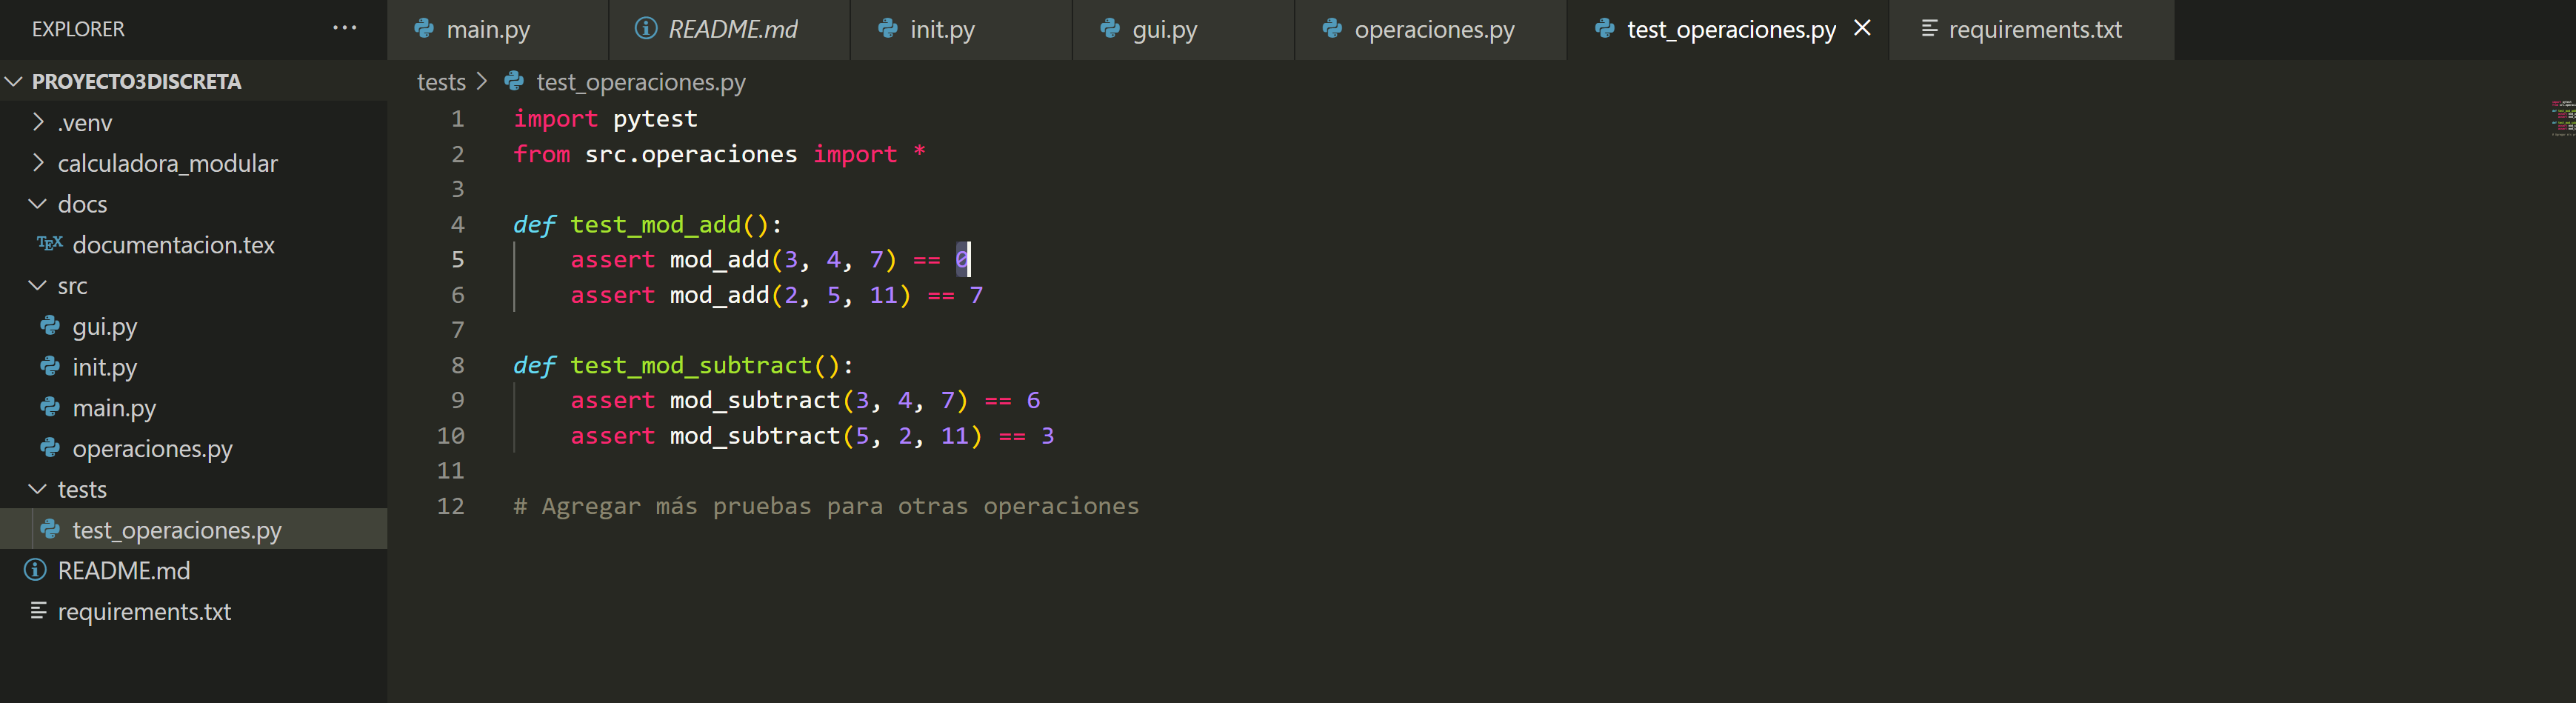
\includegraphics[width=0.8\textwidth]{Capturita1.png}




\section{Desafíos encontrados y soluciones}

Durante el desarrollo del proyecto, se enfrentaron varios desafíos:

\begin{enumerate}
    \item \textbf{Validación de entradas:} Fue necesario implementar una validación robusta para asegurar que todas las entradas fueran números enteros y que el módulo p fuera primo. Esto se resolvió creando una función de validación centralizada.
    
    \item \textbf{Manejo de errores:} Se implementó un sistema de manejo de errores utilizando try-except y logging para facilitar la depuración y proporcionar mensajes de error claros al usuario.
    
    \item \textbf{Implementación de operaciones avanzadas:} Algoritmos como el de Tonelli-Shanks para raíces cuadradas modulares requirieron una investigación adicional y una implementación cuidadosa.
    
    \item \textbf{Diseño de la interfaz gráfica:} Se tuvo que balancear la funcionalidad con la simplicidad en la interfaz de usuario. Esto se logró separando las operaciones básicas de las avanzadas en diferentes ventanas.
\end{enumerate}

\section{Conclusiones y aprendizajes}

Este proyecto ha proporcionado valiosas lecciones en varios aspectos del desarrollo de software:

\begin{itemize}
    \item \textbf{Matemáticas aplicadas:} La implementación de algoritmos de aritmética modular reforzó la comprensión de conceptos matemáticos abstractos y su aplicación práctica.
    
    \item \textbf{Diseño de software:} La separación de la lógica de negocio (operaciones modulares) de la interfaz de usuario demostró la importancia de una buena arquitectura de software.
    
    \item \textbf{Manejo de errores y logging:} Se aprendió la importancia de un buen sistema de manejo de errores y logging para facilitar la depuración y mejorar la experiencia del usuario.
    
    \item \textbf{Interfaz gráfica:} El desarrollo de la GUI con Tkinter proporcionó experiencia en la creación de interfaces de usuario simples pero funcionales.
    
    \item \textbf{Documentación:} La creación de este documento LaTeX reforzó la importancia de una buena documentación para explicar el diseño y funcionamiento del software.
\end{itemize}

En conclusión, este proyecto no solo cumplió con su objetivo de crear una calculadora aritmética modular funcional, sino que también proporcionó una valiosa experiencia en diversos aspectos del desarrollo de software y las matemáticas aplicadas.

\end{document}
